\documentclass[border = 10pt]{standalone}
\usepackage{tikz}
\usepgflibrary{shapes.gates.logic.US}
%\usetikzlibrary{arrows, shapes.gates.logic.US, calc}
\usetikzlibrary{circuits.ee.IEC}
\begin{document}


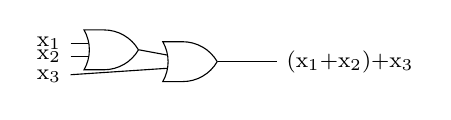
\begin{tikzpicture}
    \node[or gate US, draw, rotate=0, logic gate inputs={normal,normal}] at (1, 0) (or1) {};
    \node[or gate US, draw, rotate=0, logic gate inputs={normal,normal}] at (2, -0.15) (or2) {};
    \node (x) at ($(or1.input 1)+(-0.5,00)$) {\footnotesize x$_1$};
    \node (y) at ($(or1.input 2)+(-0.5,0)$) {\footnotesize  x$_2$};
    \node (z) at ($(or2.input 2)+(-1.5,-0.1)$) {\footnotesize x$_3$};
	\draw (x) -- (or1.input 1);
    \draw (y) -- (or1.input 2);
	\draw (z) -- (or2.input 2);
	\draw (or1.output) -- (or2.input 1);
    \draw (or2.output) -- node[right,fill=white]{\footnotesize (x$_1$+x$_2$)+x$_3$}($(or2.output)+(1.5,0)$);
    \end{tikzpicture}
\end{document}


